\section{Side Channels}
At any given moment, in the system informations are constantly flowing, because
it is an intrinsic phenomenon of computation. This is true both for a single computer system and a
distributed one.\\
Anyway, all those information flows use intended, specific and implemented channels, in which the
data requires some security guarantees, such as integrity, availability, non-repudiation, \dots\\

\begin{section}{Covert Channels}
  \begin{boxH}
    A covert channel is a path for an illegal flow of information within a system.
  \end{boxH}
  Any communication channel that a process can exploit to transfer information in a manner that
  violates the system’s security policy.

  There are many types of covert channels within a computing system, based on what the covert channel
  actually is:
  \begin{itemize}
    \item Timing covert channels
    \item Termination covert channels
    \item Probability covert channels
    \item Resource utilization covert channels
    \item Power covert channels
  \end{itemize}

  Side channels are most flexible, because they can be used for a large variety of uses, both to
  improve or undermine the security of a system.\\
  Every side channel have some defining characteristics:
  \begin{itemize}
    \item the existent, or if the channel is a potential one
    \item the bandwidth of the channel, or how much information can be transmitted
    \item how noisy it is, because informations can be distorted or lost by it
  \end{itemize}
  It is usually infeasible for realistic systems to eliminate every potential covert
  channel, so some usable techniques against them are to inject noise in the channel or monitor the
  pattern used to exploit the channel.

  \begin{subsection}{Power attacks}
    \begin{subsubsection}{Differential Power Analysis}
      \begin{boxH}
        Differential Power Analysis (DPA) is a statistical method for analyzing power consumption to
        identify data-dependent correlations.
      \end{boxH}
      It takes multiple traces (which requires more time and energy to collect) of two data sets and
      then computes the average difference of these traces. If the difference is close to zero, the
      two sets are not correlated, otherwise they are.\\
      Given enough traces, even tiny correlations can be seen, regardless of how much noise is in
      the system, since the noise will effectively cancel out during the averaging. This means that
      out of a large number of traces, the noise will be averaged out, while the signal will remain
      and be visible.

      \begin{figure}[h]
        \centering
        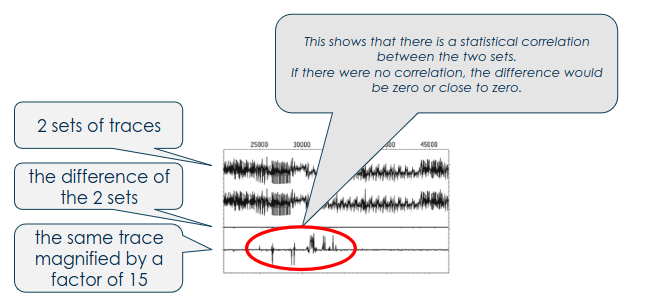
\includegraphics[width=0.5\textwidth]{dpa attack.png}
        \caption{An example of a DPA attack}
      \end{figure}
      Furthermore, this kind of attack has some benefits, in fact, even if they require some
      knowledge of the running algorithm (the physical implementation is not required), they are
      quite cheap to perform, because they need only to perform the measurements and correlate the
      power consumption of the device and the encryption data, including the key.\\
    \end{subsubsection}

  \end{subsection}

\end{section}

\begin{section}{Cache attacks}
  Cache attacks are one of the most powerful, and used one, to create a cover/side channel to exploit some
  other observations and bugs. They are based on the fact that cache are all about reducing latency
  of consecutive memory access, and because they are, mostly(eg: L1 caches), shared resources, it is
  possible to observe its state even if its not possible to directly address their memory.\\
  Many attacks uses the cache as a covert channel, like meltdown, spectre(meltdown v3), LVI(meltdown
  v4), mds(ridl/zombieload), branchscope, and many others.\\
  Different attacks exploits different features of caches, which, for the most part are:
  \begin{itemize}
    \item the cache is a shared resource
    \item the cache latency in case of miss and hit
    \item the cache associativity
    \item the cache replacement policy
  \end{itemize}
  For example the spectre attack exploits the fact that during the microarchitectural execution no
  memory boundaries are checked, in particular memory that has the same privileges, the privesc part
  is a feature of MeltdownUS/v1, and by achieving a particular memory configuration in the cache, it
  is possible to start the execution of instructions that would never be executed otherwise, because
  some required data is not available, being flushed beforehand. Than by measuring the latency of
  consecutive memory access, it is possible to retrieve the accessed data by iterating the same
  process over and over again.\\

\end{section}

\begin{section}{Cloud/FPGA Side-Channel}
  The FPGA boards can be exploited to create a covert channel, in particular the thermal and power
  to retrieve some data from the system.\\
  For example, by observing the temperature of a threshold of the FPGA, it is understand if the data
  that is being processed is a 1 or a 0, because the power consumption of the FPGA is different
  based on the data that is being processed.\\
\end{section}

\begin{section}{Side channel defenses}
  There are many approaches to defend against side channels, but the most effective one is to
  inject some noise in the channel. This is because a side channel, to be effective needs accurate
  measurements to retrieve some data, and by injecting noise in the channel, the measurements will
  be distorted, and the data will be harder to retrieve.\\
  Other approaches are:
  \begin{itemize}
    \item Leakage Reduction
    \item Key Update
    \item Side channel-resistant PUFs
    \item Secure scan chains
  \end{itemize}
  \begin{subsection}{Countermeasures against DPA}
    One of the most common is the introduction of random process interrupts. Instead of executing
    all the operations sequentially, the CPU interleaves the code’s execution with that of dummy
    instructions so that corresponding operation cycles do not match because of time shifts. The
    introduction of dummy instructions smears the peaks across the differential trace due to a
    desynchronization effect, known in digital signal processing as incoherent averaging.\\
  \end{subsection}

  \begin{subsection}{Process isolation}
    Another approach is to use process isolation techniques, like enclaves, to isolate the
    execution of a process, at the cost of hardware utilization. After all, there's no actual
    implementation that supports multi-core systems to secure the computation.
  \end{subsection}

  \begin{subsection}{Janus Cache}

  \end{subsection}

\end{section}

\end{section}
